\newpage

\section{Weryfikacja końcowa} \label{sec:weryfikacja_koncowa}

Uzyskane w trakcie badania algorytmów rezultaty pozwoliły również opracować proces potrafiący identyfikować szczyty górskie na obrazie. Z tego powodu przeprowadzono weryfikację końcową wykorzystanych metod jako całości. Odbyło się to zarówno na statycznych zdjęciach, a także w czasie rzeczywistym na kolejnych klatkach nagrań pozyskiwanych z~aparatu urządzenia mobilnego. Poniżej przedstawiono rezultaty takiej weryfikacji, a~także wyniki czasowe uzyskiwane podczas działania na żywo - w szczególności liczbę klatek na sekundę.

\subsection{Prezentacja działania rozwiązania}

Na rysunku \ref{fig:real_annotated} pokazany został przykładowy wynik otrzymany przy pomocy zaimplementowanego procesu na zdjęciu statycznym. Ze względu na gęstość szczytów na obrazie wejściowym, ograniczona została liczba naniesionych nazw, celem zwiększenia przejrzystości i czytelności. Obok nazw gór, w nawiasach została podana odległość w~kilometrach od obserwatora. 

\begin{figure}[!h]
    \centering 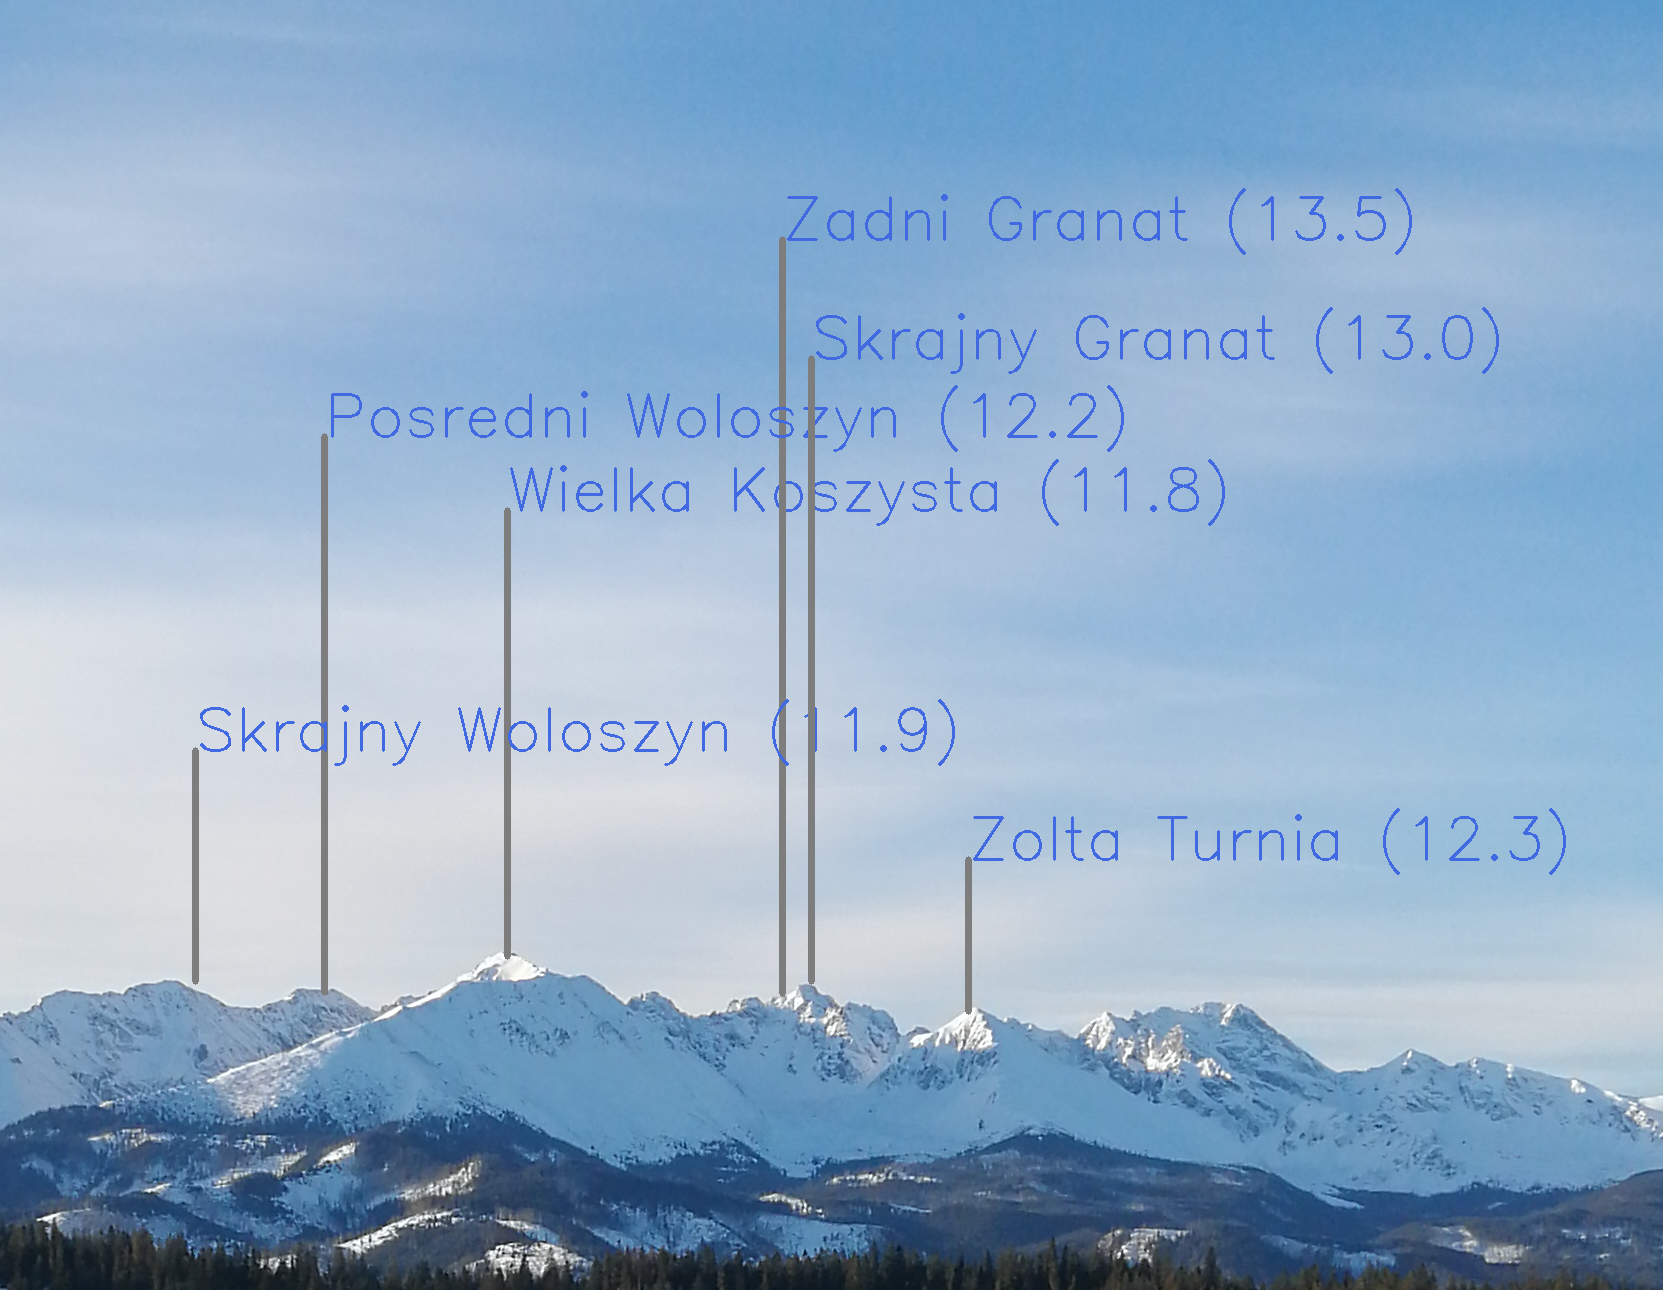
\includegraphics[width=0.65\linewidth]{img/real_annotated.png}
    \caption{Przykładowy rezultat rozpoznawania szczytów górskich na obrazie.}
    \label{fig:real_annotated}
\end{figure}


Celem demonstracyjnym przygotowano również nagrania z naniesionymi nazwami gór zrobione w paśmie Tatr, a także grafiki prezentujące wyniki kolejnych kroków procesu dla wybranych zdjęć. Opisane elementy prezentacyjne oraz kod projektu zostały umieszczone na repozytorium git autora, do którego odnośnik wraz z krótkim opisem zawartości umieszczono w załączniku 1.

\subsection{Złożoność czasowa rozwiązania}

Założeniem pracy dyplomowej było działanie algorytmów w czasie rzeczywistym. Z~tego powodu w trakcie tworzenia nagrania demonstracyjnego zebrane zostały również dane dotyczące czasu trwania procesu rozpoznawania szczytów górskich.

Pozwoliło to sprawdzić liczbę klatek generowanych przez stworzone rozwiązanie w~warunkach rzeczywistych. Przeciętnie dopasowywane było około $30$ gór, z czego $15-20$ było rozpoznanych i etykietowanych  na każdej pobranej z kamery klatce. Do testu i prezentacji wykorzystane zostało jedynie urządzenie Huaweii Mate 50 Pro. Wyniki czasu przetwarzania zostały przedstawione w tabeli \ref{tab:real-time}. Badanie wykonane było $10$ razy i trwało $1000$ klatek każde, a rezultaty uśrednione.

\begin{table}[!h]  \centering
\caption{Czas przetwarzania procesu rozpoznawania szczytów górskich na obrazie w warunkach rzeczywistych.}
\begin{tabular} {| c | c | c |} \hline
    Całkowity czas & 
    \begin{tabular}[c]{@{}c@{}} Średni czas \\ jednej klatki \end{tabular}  &
    \begin{tabular}[c]{@{}c@{}} Liczba klatek \\ na sekundę \end{tabular}
    
    \\ \hline\hline
    
    $44,9635$ s & 
    $0,044$ s& 
    22,24 FPS
    
 \\ \hline
   % \multicolumn{2}{|r|}{Suma:} & 123,45 \\ \hline
\end{tabular}
\label{tab:real-time}
\end{table}

Rozwiązanie w trakcie testu generowało $22,24$ klatek na sekundę, co wydaje się wynikiem zadowalającym. Jest to wartość zbliżona do standardu kinowego, w którym filmy na ekranie wyświetlane są z częstotliwością $24$ klatek. Z tego powodu uzasadnione jest stwierdzenie, że uzyskany rezultat oznacza wystarczający komfort użytkowania na nowszych urządzeniach mobilnych.




\subsection{Podsumowanie weryfikacji końcowej}

Przeprowadzona weryfikacja końcowa zaimplementowanego procesu identyfikacji szczytów górskich na obrazie pozwoliła stwierdzić, że uzyskane wyniki badanych i optymalizowanych algorytmów mogą być zastosowane w projektach mających na celu takie działanie. Na podstawie sprawdzonego działania rozwiązania zarówno na statycznych zdjęciach, jak i nagraniu na żywo można uznać, że w wystarczającym stopniu dokładnie opisuje ono widoczne szczyty górskie. Natomiast, rezultaty pomiaru liczby klatek na sekundę oznaczają, że rozwiązanie może zostać sklasyfikowane jako działające w czasie rzeczywistym na badanym urządzeniu.